

\tableofcontents
\newpage

\listoffigures

\chapter{Introduction}
 
 
 \section{Client Side Web Applications}
 \section{General remarks}
 \section{Structure of this Paper}
\chapter{Term Definitions}

\chapter{Analysis of Current Solutions For Developing Client Side Web Applications}
 \section{Economical and Technical Advantages of Client Side Web Applications}
 \section{Current solutions for Developing Client Side Web Applications}

  At the time of writing (first quarter of 2004), three solutions for developing client side browser based applications exist: JavaScript and Java are two platform independent options for developing the applications, Microsoft's ActiveScripting is an option for applications that only need to run on the MS Windows/Internet Explorer platform.

  \subsection{Platform Independent Solutions}
  
   \emph{As stated above, JavaScript and Java are platform independent solution, JavaScript being available on almost any modern web browser and Java as a platform independent programming language. }
   
   \subsubsection{JavaScript}
   
    JavaScript/ECMAScript\footnote{The language standardized in the ECMA-262 standard is called ECMAScript by the standard. This name came only up with the standardization of the language and never got used widly, JavaScript is still the more prominent name and will be used} is the common name for the scripting language defined in ECMA standard 262. It was originally developed
% as JavaScript 
by Brendan Eich at Netscape. The purpose of JavaScript was to give web developers the posibility create interactive HTML documents; JavaScript is integrated with Netscape's Navigator web browser since version 2.0. An alternative implementation of a JavaScript interpreter was developed by Microsoft. This interpreter however was not bound directly to Microsoft's Internet Explorer web browser but integrated into it using ActiveX/OLE/COM(?). The Microsoft JavaScript interpreter however is not fully compatible to Netscape's interpreter; the Microsoft derivative of JavaScript is called \emph{JScript}. The JScript interpreter is bundled with the Internet Explorer starting with its 3.0 release. Microsoft's approch to client side browser scripting however is not limited to JScript, section \ref{sec:activescripting} gives more information on this.

The development of the standard for the JavaScript language, standardized as ECMAScript, started in November 1996; the standard was adopted first in June 1997. It was also accepted as ISO/IEC standard 16262 in April 1998. As of February 2004, the standard is in its third edition and availabe from \cite{ECMA-262}, which correspondes to JavaScript 1.5.

%ECMA262: http://www.ecma-international.org/publications/standards/Ecma-262.htm
%	+ pdf document

JavaScript is now available -- to different extents -- in all relevant web browsers; additionally, stand-alone JavaScript interpreters exist that allow the use of JavaScript as a standalone script language not limited to in-browser use. One of the most prominent of these interpreters is the Rhino JavaScript interpreter maintained by and available from The Mozilla Organisation.

%mozilla.org, mozilla.org/rhino, availablity of JS in browsers?

For use as client side scripting language in web applications, JavaScript has some important disadvantages:

\begin{description}
	\item[Limited Possibilites] The possibilites provided by standard conform JavaScript are very limited. Java\-Script only allows interaction with its parent document\footnote{The document that embedds or references the script.}, not with any system or network ressources. Tasks that require for example file system, database or network access are not possible with standard conform JavaScript.\footnote{These limitations do not apply to Microsoft's JScript, cf. section \ref{sec:activescripting}.} 
	\item[Missing Standard Conformance] Another problem with Java\-Script based solutions is that although Java\-Script is standardized, different browsers interpret the same JavaScript code differently and any non-trivial application based on JavaScript has to be customized to the browser platform it will be used on. For an application that has to work on different platforms, for example Opera and Internet Explorer, some parts have to be coded for each browser separatly along with code deciding at run time which browser it runs on and which code is the one that must be used. A consequence of this is that JavaScript applications get overly complex and \emph{expensive} when the resulting application shall be availble on multiple browsers.
\end{description}

However, JavaScript also has some important advantages:
\begin{description}
	
	\item [Easy to Learn] JavaScript is a loose typed language, the syntax is a mix of elements from C and Java and a lot of simple examples and tutorials is available for free on the web.\footnote{E.g. at \cite{W3SchJS}} Additionally, nothing but a web browser is necessary to start programming with JavaScript.
	
	\item [Wide User Base] JavaScript is integrated in all relevant browsers and thus provides a wide user base that can use JavaScript applications 'out of the box'. As JavaScript is always available when a web browser is installed,, no costs of maintaining or installing JavaScript accumulate.
	
	\item [Secure] As JavaScript implementations conforming to the standard do not allow operations outside of their designated are -- their parent document -- potentially hazardous actions like reading content from other browser windows or accessing the local file system are theoretically not possible.\footnote{This does not to the JScript security model, cf. section \ref{sec:activescripting}.}
	
\end{description}
    
   \subsubsection{Pure Java}
   
    Java is an object oriented programming language developed by Sun and available since 1995. Java, from the beginning of its development, was designed to be a platform independent programming language: The concept of Java consists of a 'two-step' approach in compiling and running Java programs: The Java source code is compiled into a architecture neutral bytecode; upon running, that bytecode is interpretet by the Java virtual machine that must be available on the computer running Java application.

One of the most important reasons why Java was created platform independant was the intention to use Java as a programming language in heterogenous environments, especially the internet, where platform independence make it possible to write applications once and run them on any desired platform.

%JAVA PLUGIN

Another feature of Java is that it allows the creation of applications that can be embedded in HTML documents: Java applets. These applets reside in and control a designated area of the HTML document. As Java, in contrast to JavaScript, is a full featured language, these applets could potentially be dangerous. To allow the use of Java applets without compelling users to check the security of the applets, Java created a secure environment, the sandbox, for Java applets that allows only safe operations; in order to allow potentially harmful tasks like filesystem access, this sandbox can be left when the user explicitly allows this. The security model of the Java sandbox is fine-grained, the user can specify exactly which applet should have which permission (which files may be accessed, which hosts contacted over the internet, ...). 

The Java Standard Edition comes with hugh class library that provides classes for most standard tasks like reading files from local and remote locations, database access or TCP/IP connections. All of this functionality is available in Java applets.


Current versions of the Java plugin also allow applets access to elements of browser documents. 

However, compared with JavaScript, interaction with document elements is much more complicated. 




In a nutshell, the disadvantages of Java are:

\begin{itemize}
	\item It is much harder to learn than most scripting languages.
	\item Interaction between Java and web browsers is more complicated than it is with 'browser native' languages.
	\item Java code must be compiled, it can not be changed at runtime.
	
\end{itemize}

Advantages of Java are:

\begin{itemize}
	\item Java is a truely platform independent programming language available on all major operating system and hardware platforms.
	\item Java comes with a huge class library.
	\item Program execution is much faster than it is with scripting languages.
	\item Java code distributed over the internet runs in a safe environment.
\end{itemize}
    
  \subsection{A Proprietary Solution: Microsoft ActiveScripting}
  \label{sec:activescripting}
    
   ActiveScripting, also called ActiveX Scripting, is a technology developed by Microsoft that can be used for client side scripting in web browsers. It is a proprietary solution available only for the Microsoft platform, that is for the Windows operating systems and the Internet Explorer web browser.

ActiveScripting is based on COM interfaces that can be used to communicate with the various supported scripting engines. It is not limited to a specifig scripting language, instead scripting engines for various languages are available from Microsoft and other vendors, see table  \ref{tab:ActiveScriptingEngines} for an overview of some available languages.\footnote{Developing a scripting language for languages other than these is possible, information on this is available at \cite{MsCreateSE}.}

%ref MsCreateSE: http://msdn.microsoft.com/library/default.asp?url=/library/en-us/script56/html/scripting.asp

\begin{table}[hb]
	\centering
		\begin{tabular}{ll}
			\textbf{Language}& \textbf{Vendor} \\
			& \textbf{URL} \\
			VBScript & Microsoft \\
			& \texttt{http://www.microsoft.com/scripting/vbscript/} \\
			JScript & Microsoft \\
			& \texttt{http://www.microsoft.com/scripting/jscript/} \\
			Perl & ActiveState \\
			& \texttt{http://www.activestate.com/Products/ActivePerl/}\\
			Python & Python.org \\
			&\texttt{http://www.python.org/windows/win32com/ActiveXScripting.html} \\
		%	Haskell & \sffamily http://www.haskell.org/haskellscript \\
			Object Rexx & IBM \\
			& \texttt{http://www-306.ibm.com/software/awdtools/obj-rexx/}\\
			
		\end{tabular}
	\caption{Active Scripting Engines}
	\label{tab:ActiveScriptingEngines}
\end{table}


Used as a client side web scripting language, some of the advantages of ActiveScripting are:

\begin{description}
	
	\item [Language Independent] ActiveScript not depending on a specific programming language developers must use; instead, it provides the possibility to choose one of several available languages like JScript, VBScript or Perl.
	
	\item [Powerful] ActiveScripting languages are based on the windows COM and can therefore use all parts of a system that provide COM interfaces, including system ressources and most Windows applications.
	
	\item [Easy to Use] ActiveScripting languages can access the DOM of HTML documents works exactly as this works using standard JavaScript scripts\footnote{Microsoft's JScript itself is an ActiveScripting language.}, the \emph{learning barrier} to using non-JavaScript languages in HTML environments is very low.

\end{description}

In contrast to these advantages, ActiveScripting also has some severe disadvantages:

\begin{description}
  
  \item [Insecure] ActiveScripting within HTML documents can only be switched on or off\footnote{The decision if scripting shall be allowed can be made based on signatures and URLs.}, a differentiated approach to allow or prohibit specific actions of a script is not possible. It also is impossible to run scripts in a secure environment similar to the Java sandbox.
  
  \item [Platform Dependence] ActiveScripting is limited to the Microsoft Windows/Internet Explorer platform and thus the creation of applications based on this technology creates massive lock-in effects and raises switching costs to other platforms as solutions based on this platform would have to be rewritten at least partially.
  
\end{description}
     
\chapter{BWS}

 BWS is an approach to integrate some existing technologies (see section \ref{sec:BaseTechnologies}) into one solution for developing platform independent client side scripted HTML/XML documents.

 \section{Technical Overview}
  
  Technically, BWS is split in two parts: The first one transforms a BWS document meeting the requirements stated in section \ref{sec:XHTMLDocumentsAsStartingPoint} to a browser interpretable HTML document the second one provides the runtime environment that connects the different technologies necessary for script execution and DOM integration.

\begin{figure}[htbp]
	\centering
		\includegraphics[scale=0.70]{technologicalOverview}
	\label{fig:TechnicalOverviewOfBWS}
	\caption{Technical Overview of BWS}
\end{figure}

As depicted in figure \ref{fig:TechnicalOverviewOfBWS}, the first part of BWS, document rewriting, can be integrated into the second one so that working with BWS document for the user is no different to working with conventional HTML documents.
  
 \section{Base Technologies}
 \label{sec:BaseTechnologies}
  
  The technologies used in BWS are the Document Object Model (DOM), Java DOM communication with LiveConnect and the Java Plugin, and the Bean Scripting Framework (BSF).
  
  \subsection{DOM}
  
   The DOM 
\begin{quotation}
	is a platform- and language-neutral interface that will allow programs and scripts to dynamically access and update the content, structure and style of documents.\footnote{w3dom,whatis}
\end{quotation}
%ref http://www.w3.org/DOM/#what

It is standardized by the W3C DOM working group which accepts submissions from member companies and tries to implement their wishes in a interoperable and scripting-language neutral solutions.

   
   \subsubsection{DOM Basics}
   
    
DOM objects are hierarchically organized into a DOM tree with the topnode of a XML document as the root object of the DOM tree. Every part of a XML document correspondes to a DOM object: The following code snippet of a XML document is mapped to the tree shown in figure \ref{fig:simpleDomTree}.

\begin{verbatim}
<html>
 <head>
  <title>DocumentTitle</title>
 </head>
 <body>
  <h1 id="aHeading">Heading</h1>
  <br />
  <p id="aParagraph" style="fontFamily:sans-serif;">Content</p>
 </body>
</html>
\end{verbatim}

\begin{figure}[htbp]
	\centering
		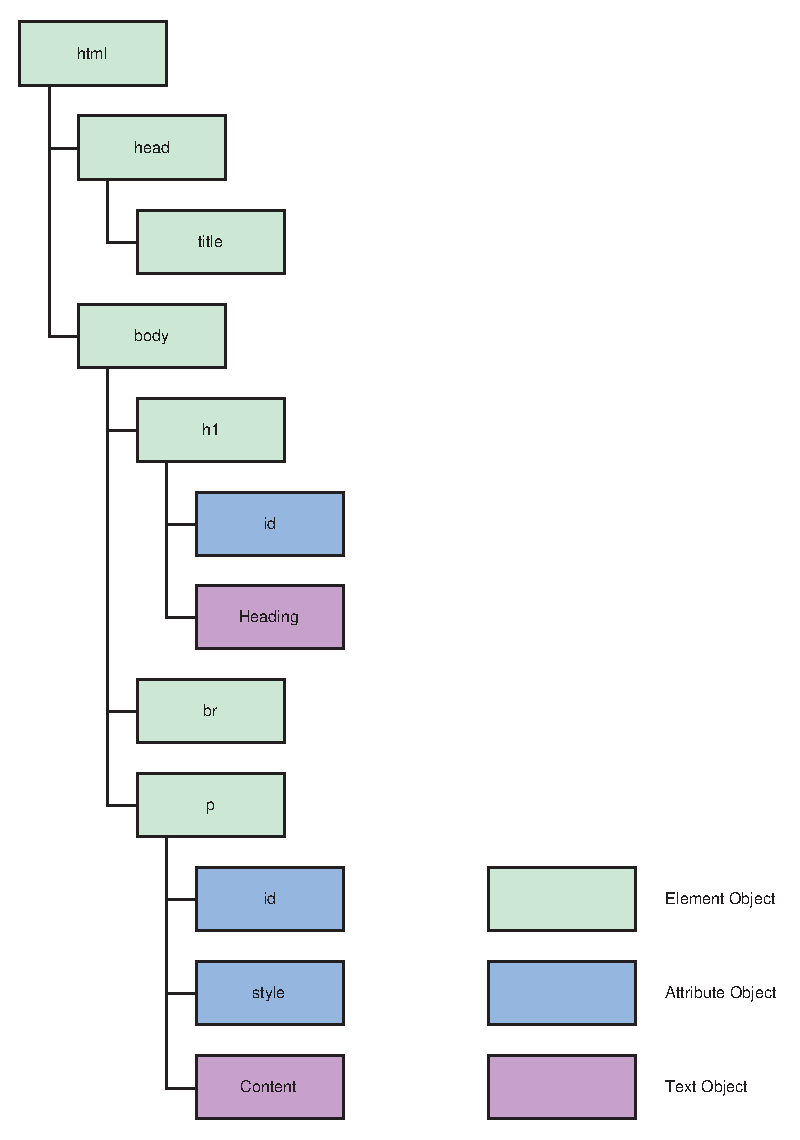
\includegraphics[scale=0.5]{simpleDomTree}
	\caption{SDT}
	\label{fig:simpleDomTree}
\end{figure}

The figure showes three types of DOM 'classes': 

\begin{enumerate}
	\item Element objects, these correspond to XML tags and are characterized by there type, e.g. a \texttt{h1} or a \texttt{title}.
	\item Attribute objects, these correspond to XML attributes and are name-value pairs, e.g. the paragraphs \texttt{style} value is \texttt{Heading}.
	\item Text objects, the part of the document between the tags that is the (unstructured) content of document.
	
\end{enumerate}

Properties and methods available for these DOM classes are also definined in the DOM standard; DOM for example defines that each element node may have an attribute \texttt{id} and that every element node supports the method \texttt{appendChild} that expects another node as argument and attaches this node to the node the method is invoked on.


    
   \subsubsection{DOM in Java: dom4j}
    
    In order to work with these objects, it is necessary that they are available in the programming language used; in this case this is Java.

One of the solutions available for mapping DOM objects to Java objects is the open-source solution dom4j. This framework enables the parsing of XML documents to Java objects, the navigation and modification of parts of the represented XML document as well as the creation of a XML document from the Java objects.

dom4j provides two ways of accessing the Java objects corresponding to a specific DOM element: The first one is to walk the DOM tree hierarchically that is, iterate over all elements of the lowest layer, check if one of the elements of this layer match the desired criteria, then select all of the elements of the next lower layer and do the same for all layers until the desired element is reached. 

For example if in figure \ref{fig:simpleDomTree} the heading's content is wanted, the procedurce would have to look like this:

\begin{enumerate}
\item Select all child elements of the \texttt{html} node.
\item Check if the elements type is \texttt{body}.
\item If it is \texttt{body}, select all child elements of this element.
\item Iterate over these elements and check if they are \texttt{h1} elements.
\item If a element is a \texttt{h1}, select its content.
\end{enumerate}

As this method is very laborious and time consuming, especially for complex and large XML documents, dom4j provides another way of selecting the desired elements: the XML Path Language (XPath).

    
   \subsubsection{Selecting DOM Elements: XPath}
   \label{sec:SelectingDOMElementsXPath}
    XPath, standarized by the W3C is a XML element query language: It allowes to specify certain criteria that are then used to select all elements of a XML document that match these criteria. The easiest way is specifying the path to an element, to address the \texttt{h1} element in figure \ref{fig:simpleDomTree}, the apropriate XPath expression would be \verb|/html/body/h1|, that is, the root element (\verb-/-) and all relevant children types separated by (forward) slashes.

For selecting the \texttt{h1} content, the procedure would be this:

\begin{enumerate}
	\item Select the \texttt{h1} element with XPath using \verb|/html/body/h1|.
	\item Get this element's content.
\end{enumerate}

However, this way of selecting elements is still based on the full path of the elements within the DOM tree and does not allow accessing elements only by type (without specifying a full path). For this purpose, XPath provides the posibility to select elements independent from their path. XPath expressions using this method start with a double slash (\verb|//|) instead of the single root slash. The expression for selecting all \texttt{h1} elements in a document therefore would be \verb|//h1|.

This would allow to use the following procedure for selecting the \texttt{h1} content:

\begin{enumerate}
	\item Select all \texttt{h1} elements with XPath using \verb|//h1|.
	\item Get all selected elements' content.
\end{enumerate}

The difference between the two examples using XPath above is that the second example would return any \texttt{h1} element within the document independant of its position (i.e. it would also return a \texttt{h1} lying under the \texttt{p} element in the given document whereas the first expression would only reply \texttt{h1} elements that are exacly in the third layer of the document and have \texttt{html/body} as parents.
   
   \subsubsection{Modifiying the DOM in Java with dom4j}
   
    The first step in modifying an existing\footnote{dom4j also provides the possibility to build DOM trees/XML documents form scratch. As this possibility is not used in BWS, it is not \emph{detailed} in this paper.}  DOM in Java is parsing the DOM underlying XML document and building the DOM tree in Java. dom4j uses the Simple API for XML (SAX)\footnote{SAX is available from \cite{SaxHP}} for this purpose.

%saxhp=www.saxproject.org

Reading the XML document is done by using a \texttt{org.dom4j.io.SAXReader} objects \texttt{read()} method on the source of the XML document; the source may be a \texttt{String}, an \texttt{URL}, a \texttt{InputStream}, a \texttt{Reader} or a \texttt{org.sax.InputSource}. This method returns a DOM tree as an \texttt{org.dom4j.Document}.

The root element of the parsed document can then be obtained using the \texttt{getRootElement()} method on the document returned from the \texttt{SAXReader}. Elements in dom4j are objects of the class \texttt{org.dom4j.Element}.

To allow access to child elements of the current element, each \texttt{Element} provides a standard Java \texttt{Iterator} that allows iteration over all child objects. Figure \ref{fig:AMinimalDom4jExample} shows a minimal dom4j example that provides two methods: \texttt{parseDocFromURL()} to read an XML document from an URL and \texttt{printRootChildren()} to print the element types of all direct child nodes of the root element of the document read with the \texttt{parseDocFromURL()} method.

\begin{figure}[htb]
  \begin{verbatim}
import java.util.Iterator;
import java.net.URL;

import org.dom4j.*;
import org.dom4j.io.SAXReader;

public class Dom4jExample {
  private Document dom4jDocument;
  
  /* SAXReader.read() throws a DocumentException when problems reading
   * or parsing an XML document occur, for example if the document is
   * not available at the specified place or if it is not well-formed.
   */
  public void parseDocFromURL(URL anURL) throws DocumentException {
    SAXReader xmlReader = new SAXReader();
    this.dom4jDocument = xmlReader.read(anURL);
  }
  
  public void printRootChildren() {
    Element documentRoot = this.dom4jDocument.getRootElement();
    
    Iterator elementIterator = documentRoot.elementIterator();
    
    // iterate over all children
    while(elementIterator.hasNext()) {
      Element currentElement = (Element)elementIterator.next();
      System.out.println(currentElement.getName());
    }
  }
}
  \end{verbatim}
	
	\caption{A minimal dom4j example}
	\label{fig:AMinimalDom4jExample}
\end{figure}
    
  \subsection{LiveConnect and the Sun Java Plugin}
  
   LiveConnect was the first technology that allowed interaction betwwen Java, JavaScript and scriptable browser plugins. It enables calls of Java methods from JavaScript as well as access from Java to the functionality of JavaScript.

The development for Java/JavaScript interaction was started by Netscape Inc. in 1996; it was first availablel with the release of the Netscape Navigator 3.0. Nowadays \footnote{February 2004.} this functionality is provided by the Sun Java Plugin.

For this Java/JavaScript interaction, Netscape provides the \texttt{netscape.javascript.JSObject} Java class that capsules all non-primitive data types passed between JavaScript and Java. This class also provides the only way for Java to access the current documents DOM\footnote{From Java 1.5 on, Sun \emph{will provide} another, better adjusted possibility for accessing the DOM called the \emph{Common DOM API}}. Due to this very generic DOM interface, modifiying the DOM from Java is comparativly elaborate. See figure \ref{fig:JavaJSDomAccess} for a comparison of modifiying a DOM element from Java compared to modifying it from JavaScript.

\begin{figure}[htbp]
Setting the background color of the first heading to red in JavaScript and Java.	
\begin{verbatim}
firstHeading=window.getElementsByTagName("h1")[0];
firstHeading.style.backgroundColor="red;"
\end{verbatim}
JavaScript

\begin{verbatim}
Object[] objectArray=new Object[1];
JSObject appletWindow=this.getWindow();
objectArray[0]="h1";
JSObject headingArray=
  (JSObject)appletWindow.call(getElementsByTagName,objectArray);
JSObject firstHeading=(JSObject)headingArray.getSlot(0);
JSObject styleAttribute=(JSObject)firstHeading.getAttribute("style");
objectArray[0]="red";
styleAttribute.setMember("backgroundColor",objectArray)
\end{verbatim}
Java

	\caption{Comparision of DOM access in Java and JavaScript}
	\label{fig:ComparisionOfDOMAccessInJavaAndJavaScript}
\end{figure}
   
  \subsection{BSF}
  
   The Bean Scripting Framework (BSF) is

\begin{quotation}
	a set of Java classes which provides scripting language support within Java applications. It also provides access to Java object and methods from supported scripting languages.\footnote{\cite{BsfFaq}}
\end{quotation}
%ref BsfFaq: http://jakarta.apache.org/bsf/faq.html#what-is-bsf

The main accent of BSF usage at the moment\footnote{February 2004} is the use of scripting languages within JSPs and to allow these scripting languages access to the Java class library. Additionally, BSF enables the creation of Java applications complete or partially in scripting languages. To enable these possibilities, BSF provides an API that allows the invokation of scripting engines from Java and an central object registry, the BSF registry, that allows to register object \emph{that are then} available for the scripts called.

BSF was initally developed at an IBM research center with the motivation to provide access to JavaBeans from scripting languages. It was moved to IBM's AphaWorks\footnote{Cf. \cite{IbmAlpha}} site\footnote{A website whereon IBM provides developers access to its latest inovations} where it found significant interest. This led IBM to move it on to its developerWorks\footnote{developerWorks `is IBM's technical resource for developers'\cite{IbmDevelAbout}; it provides technical information and code for developers using IBM and open standards technologies like WebSphere, DB2, Java, Linux, etc.}  site\footnote{Cf. \cite{IbmDevel}} where it was developed as an Open Source project until the release of BSF 2.2. BSF was incorporated into IBM's application server WebSphere\footnote{http://www.ibm.com/websphere} and also into the Xalan XSLT processor developed by the Apache project.
%ref IbmAlpha: http://alphaworks.ibm.com/, http://alphaworks.ibm.com/about
%ref IbmDevel: http://www.ibm.com/developerworks
%ref IbmDevelAbout: http://www.ibm.com/developerworks/aboutdw/

The interest of the Apache project in BSF finally led IBM to hand over the project to the Apache foundation where it is developed since 2002 as an subproject of Jakarta\footnote{\textbf{What is Jakarta?}}. As of February 2004, the current release of BSF is 2.3.

\subsubsection{BSF Architecture}

For consists of two primary components, the \texttt{BSFManager} and the \texttt{BSFEngine}. The \texttt{BSFManager} maintains the BSF object registry and handles the scripting engines. To use the BSF, a Java application must instanciate a \texttt{BSFManager} and then either load a scripting engine directly using the \texttt{BSFEngine} interface or indirectly using the \texttt{BSFManager} as a proxy. The \texttt{BSFManager} also caches scripting engines so these only have to be instanciated once.

The \texttt{BSFEngine} interface represents a single scripting engine. Scripting engines are returned by a \texttt{BSFManager}'s \texttt{loadScriptEngine()} method and can then be used to execute scripts passed to them.\footnote{Cf. \cite{BsfManual}.}
%ref http://jakarta.apache.org/bsf/manual.html

For an overview of the structure of BSF and the two methods of executing scripts see figure \ref{fig:bsfOverview}.

\begin{figure}
	\centering
		\includegraphics[width=0.90\textwidth]{bsfOverview}
	\caption{BSF Overview}
	\label{fig:bsfOverview}
\end{figure}

An overview of the methods provided by BSF is available at \cite{BsfManual}.

\subsubsection{BSF4Rexx}

BSF4Rexx enables the binding of several rexx interpreters\footnote{Classic Rexx, Object Rexx and Regina} to the BSF an thus provides a Rexx scripting enginge. BSF4Rexx was developed initially by Peter Kalender, a student at the University of Essen, in the winter semester of 2000/2001, for a term paper. \cite{Kale00}
% Kale00 http://nestroy.wi-inf.uni-essen.de/Lv/seminare/ws0001/PKalender/Seminararbeit.pdf
BSF4Rexx has since been extendend and is maintained by Prof. Rony Flatscher of the WU Wien; it is available from \cite{BSF4Rexx},
%BSF4Rexx http://wi.wu-wien.ac.at/rgf/rexx/bsf4rexx/
a detailed article on BSF4Rexx is \cite{Flat01}.
%Flat01 http://wi.wu-wien.ac.at/rgf/rexx/orx12/JavaBeanScriptingWithRexx_orx12.pdf
  
  \subsection{Relations Between the Base Technolgies}
   
   The technologies described above are used in BWS in the following relations:

For document rewriting, dom4j is used to transform the user created BWS document to a Java object tree. Using other methods provided by dom4j, these objects are then modified to represent a browser interpretable document. This resulting object tree is then \emph{written out as a HTML document}.

During execution of the document, LiveConnect is used to provide DOM access to the runtime environment applet, BSF is used to run the scripts and forward their DOM. For a graphical representation see figure \ref{fig:TechnicalOverviewOfBWS}.
   
 \section{Classes and Their Relations}
 
  BWS consists of two separted sets of classes: 

\begin{itemize}

\item The first set is based on the \texttt{BWSDocument} class that represents an BWS document and provides methods to transform it to a browser   interpretable HTML document and is used by the \texttt{BWSRewriter} and the \texttt{BWS2XHTML} class.
 \texttt{BWSRewriter} reades the BWS document from an URL specified on the command line, rewrites the document and
 prints messages useful for debugging a failing document; \texttt{BWS2XHTML} also reades the document from a specified
 URL and prints only the transformed document to the standard output.

\item The second set is based on the \texttt{BWSApplet} class that provides the runtime environment for BWS scripts. This class utilizes the \texttt{JSNode} class, a capsule class for the HTML/XML nodes\footnote{Independent of the node type, i.e. element, text and attribute nodes, just as the DOM's \texttt{node} 'class' does.}, and the \texttt{ScriptString} class that is used for the interpretation and evaluation of script calls from events.

\end{itemize}

Figure \ref{fig:bwsDocumentRepresentation} shows which elements of a document are represented by which classes, figure \ref{CREATETHISFIGURE} shows the relations between the classes and their relations to the classes of external packages.

\begin{figure}
	\centering
		\includegraphics[width=0.90\textwidth]{bwsDocumentRepresentation}
	\caption{BWS Documents - Representation in Java}
	\label{fig:bwsDocumentRepresentation}
\end{figure}

   
 \section{BWS in Action}
  
  The following section will describe the two parts of BWS in detail as they are implemented.
  
  \subsection{Details of Document Rewriting}

   Document rewriting is the process of rewriting a BWS document conforming to the requirements defined in section \ref{sec:CreatingBWSApplications} to HTML documents interpretable by the browser. To achieve this, BWS script calls must be transformed to JavaScript calls calling Applet methods and the BWS runtime environment, the \texttt{BWSApplet} class, must be embedded in the document. As shown if figure \ref{fig:TechnicalOverviewOfBWS}, this process can be run separatly from the application execution itself or it can be run inside the BWSApplet; then of course the applet must be embedded beforehand by the creator of the BWS document.

   \subsubsection{BWSDocument class}
    
    The \texttt{BWSDocument} class is, as shown in figure \ref{fig:bwsDocumentRepresentation}, a Java representation of a BWS document. It provides methods for transforming a BWS document to a browser interpretable HTML document by rewriting the script calls from BWS script calls to JavaScript calls of an applet method that in consequence runs the desired script. Additionally, it embedds the runtime environment applet in the HTML document.

For these purposes, the class provides six methods, for an overview see the class diagram in figure \ref{fig:classDiagrammBWSDocument}. The \texttt{printDocumentSource()} method an the \texttt{printVector()} method are useful for debugging the BWS document, the other methods are used for rewriting the document.

\begin{figure}
	\centering
		\includegraphics{classDiagrammBWSDocument}
	\caption{Class diagram: \texttt{BWSDocument}}
	\label{fig:classDiagrammBWSDocument}
\end{figure}

The usual workflow for transforming documents is as follows:

\begin{enumerate}
	\item Read and parse the document.
	\item Gather all script ids occuring in the document.
	\item Search all attributes of all elements if they reference a BWS script and replace the script call if this it the case.
\end{enumerate}

This workflow correspondes to the following method calls of \texttt{BWSDocument}:

\begin{enumerate}
	\item \texttt{readDocumentFromURL(String URL)}
	\item \texttt{getScriptNames()}
	\item \texttt{rewriteScriptCalls()}
\end{enumerate}

The \texttt{readDocumentFromURL()} method is quite simple, it creates an \texttt{URL} and a \texttt{SAXReader}. The \texttt{SAXReader}'s \texttt{read()} method is the used on the \texttt{URL} and its result is assigned to the \texttt{xmlDocument} property of \texttt{BWSDocument}.

\texttt{getScriptNames()} is the method used for reading all occuring script names from the document. It creates a \texttt{XPath} object selecting all script elements.\footnote{The XPath expression for this is \texttt{//script}, see section \ref{sec:SelectingDOMElementsXPath}, p. \pageref{sec:SelectingDOMElementsXPath}.} This \texttt{XPath} is then used to select the matching nodes which are referenced in the \texttt{results List}. Using an \texttt{Iterator}, all scripts are parsed for their \texttt{id} attribute. The value of the \texttt{id} attribute is then added to the \texttt{scriptNames Vector}-.\footnote{A private property of \texttt{BWSDocument}.} If an \texttt{id} is not available, the \texttt{name} attribute is used instead, if this also is missing, the script is ignored.

\texttt{rewriteScriptCalls()} is a very short method that iterates over the \texttt{scriptNames Vector} and calls the \texttt{getAttributeElement()} method for each of the \texttt{Vector}'s elements.

\texttt{getAttributeElement()}
 takes a 
 \texttt{String}
  as an argument; it creates a 
  \texttt{XPath} object that selects all elements having an arbitrary attribute of the value 'bws:PassedString' or '\#:PassedString'.\footnote{
  The XPath expression for this is \texttt{//*[@*='\#:ScriptId'] | //*[@*='bws:ScriptId']} where ScriptId is the string that was passed to the \texttt{getAttributeElement()} method from the caller. The expression consists of two parts connected with the 'or' operator  (\texttt{|}),one for attribute values starting with '\#', the other one for those starting with 'bws:'; the \texttt{//*} denominates that all elements shall be searched, \texttt{@*} indicates all attributes shall be searched.
  }

After the results of this XPath expression are stored to the \texttt{List results}, an \texttt{Iterator} is created that iterates over all found elements. For each element, its attributes are stored to another \texttt{List}, \texttt{elementAttributes}. Another \texttt{Iterator} is created for this \texttt{List} and each attribute is tested if it was the one matching the XPath expression. If this is the case, the attribute value is changed to \textbf{INSERT THE REAL VALUE HERE!}.

\textbf{INSERTING THE APPLET}

The resulting final document that is stored in the \texttt{BWSDocument}'s \texttt{xmlDocument} can then be printed out to the standard output using the \texttt{printDocumentSource()} method.
     
   \subsubsection{Using BWSDocument}
    \paragraph{Server-side}
    \paragraph{Client-side}
   \subsection{Details of Application Execution}
    \subsubsection{BWSApplet}
    \subsubsection{ScriptString Class}
    
     \texttt{ScriptString} is the class providing interpretation of BWS script call strings for the runtime environment. These call strings are the strings used in DOM event handlers to call BWS scripts\footnote{An example for such a string is \texttt{returnValue=scriptId(parameter1,parameter2)}.}. These strings are passed to the \texttt{BWSApplet} using the \texttt{executeScript()} method and then have to be interpreted by the applet/runtime enviroment to call the appropriate script, lookup the specified parameters and store the return value to the specified place after script execution. A class diagram of the \texttt{ScriptString} class is depicted in figure \ref{fig:classDiagramScriptString}.

\begin{figure}[htbp]
	\centering
		\includegraphics{classDiagrammScriptString.eps}
		\caption{Class Diagram: \texttt{ScriptString}}
	\label{fig:classDiagramScriptString}
\end{figure}

The \texttt{get*} methods of this class provide other classes access to the result of the interpretation. The interpretation itself is done in the \texttt{ScriptString} constructor\footnote{\emph{I know this is plain evil!}} using the \texttt{parseParameters()} method to interpret the parameter part of the string.
     
    \subsubsection{JSNode Class}
    
     JSNode class documentation
     
     \paragraph{JSNode Method Overview}
     
      

A \texttt{JSNode} object can be constructed using one of three available constructors, see table \ref{tab:JSNodeConstructors}.

\begin{table}[htbp]
	\centering
		\begin{tabular}{ll}
			\textbf{Method Head} & \textbf{Description} \\
			\texttt{JSNode(JSObject window,} & Creates a reference to the node with the \texttt{id nodeRef}\\
			\texttt{ String nodeRef)}&  in the \texttt{window}.\\
			
			\texttt{JSNode(JSObject window,}& Creates a reference to the node passed as \texttt{existingNode}.\\
			\texttt{ JSObject existingNode)}& \\
			
			\texttt{JSNode(JSObject window,}& Creates a reference to the node passed as \texttt{exitingNode}\\
			\texttt{ JSObject existingNode,}&  and sets its \texttt{id} to the specified \texttt{id}.\\
			\texttt{ String id)}& \\
		\end{tabular}
	\caption{JSNode Constructors}
	\label{tab:JSNodeConstructors}
\end{table}

Additionaly, a node can be obtained without specifing a window calling an existing \texttt{JSNode}'s \texttt{getJSNode()} method. This method expects a reference to a existing node of the type \texttt{JSObject} as its argument. It returns a new JSNode with the window of the called node.

%texttt{JSNode} also provides methods

Other methods provided by \texttt{JSNode} can be used to obtain the nodes window (\texttt{getWindow()} and document (\texttt{getDocument()}), its \texttt{id}(\texttt{getIdentifier()}), the full content in HTML of an element (\texttt{getInnerHTML()}) and the node object referenced by the \texttt{JSNode} (\texttt{getNode()}).

\texttt{JSNode} also provides three methods for creating new nodes of different types:

\begin{itemize}
	\item \texttt{createAttribute(String attributeType, String attributeValue)}, creates an attribute named \texttt{attributeType}, e.g. \texttt{style} or \texttt{name}, set to the value \texttt{attributeValue}.
	\item \texttt{createElement(String elementType)}, creates an element of the type \texttt{elementType}, e.g. \texttt{h1} or \texttt{div}.
	\item \texttt{createTextNode(String elementText)}, creates a text node with the specified content (\texttt{elementText}).
\end{itemize}


      
     \paragraph{Advantages of JSNode Over Conventional LiveConnect DOM Access}
     
      The purpose of \texttt{JSNode} is to ease the access to DOM elements at runtime in comparision to LiveConnect. As LiveConnect handels all DOM interaction over \texttt{JSObject} which provides very limited functionallity, DOM interaction only using LiveConnect directly usually leads to long and error-prone code. Especially when compared to JavaScript DOM interaction, direct Java DOM interaction is unnecessary complicated.\footnote{Cf. figure \ref{fig:ComparisionOfDOMAccessInJavaAndJavaScript}}. 

One of the most problematic and 'code-consuming' problems with \texttt{JSObject} is the \texttt{JSObject}'s \texttt{call()} method. This method can be used to call methods of the underlying DOM node in Java, for example, it can be used to call a nodes \texttt{getAttributeNode()} method. The syntax for calling these DOM methods is \texttt{nodeObject.call(methodName, arguments)} where \texttt{methodName} is a string representing the name of the method to be invoked, e.g. "getAttributeNode" and \texttt{arguments} is an array of \texttt{Object}s that contains the arguments that are to be passed to the method. This means that for every DOM method call, an \texttt{Object} array has to be created and the individual argument have to be saved to this array. If an argument is a primitive value, it additionaly has to be converted to an object before it can be put in the array. 

To overcome these drawbacks of 'pure' LiveConnect, \texttt{JSNode} capsules the methods normally used in JavaScript using the DOM node object. This capsuling is implemented using the methods provided by LiveConnect's \texttt{JSObject}. An example of how these methods are implemented is given in figures \ref{fig:ImplementationGetAttributeNode} and figure \ref{fig:ImplementationSetStyleAttribute}.\footnote{Debug messages were omitted in this examples to improve comprehensibility.}

The \texttt{getAttributeNode()} method expects a string that identifies the desired attribute, e.g. the \texttt{name} attribute, and returns this attribute as a \texttt{JSNode} object. To do this, \texttt{getAttributeNode()} first creates a new \texttt{Object} array with one field and assignes this field the string that was passed as \texttt{attributeName}. It then calls the \texttt{call()} method of the \texttt{JSNode}'s \texttt{node} property to obtain a \texttt{JSObject} representation of the attribute node. This \texttt{JSObject} represention is assigned to the \texttt{attributeNode} variable that is then used to create a new \texttt{JSNode} containing the \texttt{attributeNode}. This \texttt{JSNode} is then return to the calling function.

\begin{figure}[htbp]
 \begin{verbatim}
public JSNode getAttributeNode(String attributeName) {
  Object[] callArgs=new Object[1];
  callArgs[0]=attributeName;
  JSObject attributeNode=(JSObject)node.call("getAttributeNode",callArgs);
  JSNode attributeJSNode=this.getJSNode(attributeNode);
  return attributeJSNode;
}
 \end{verbatim}
	\caption{Implementation getAttributeNode()}
	\label{fig:ImplementationGetAttributeNode}
\end{figure}

\texttt{setStyleAttribute()} is a shorter method as it does not involve calling the \texttt{JSObject}'s \texttt{call()} method and thus creating and \emph{filling} an \texttt{Object} array is not necessary here. The method expects two strings, \texttt{styleAttribute} specifying the attribute that is to be set, e.g. \texttt{fontFamily} or \texttt{color}, and \texttt{value} specifying the value this attribute shall be set to.

\begin{figure}[htbp]
	\begin{verbatim}
public int setStyleAttribute(String styleAttribute, String value) {
  JSObject styleNode=(JSObject)node.getMember("style");
  styleNode.setMember(styleAttribute,value);
  return 0;
}
	\end{verbatim}
	\caption{Implementation setStyleAttribute}
	\label{fig:ImplementationSetStyleAttribute}
\end{figure}
     
\chapter{Discussion}

\chapter{Using BWS}

 \section{An Example of BWS in Action}
 \section{Installing BWS}
 \section{Creating BWS Applications}
 \label{sec:CreatingBWSApplications}
 
  \subsection{XHTML Documents as Starting Point for BWS Applications}
  \label{sec:XHTMLDocumentsAsStartingPoint}

   The starting point of a BWS compliant document is a standard well-formed HTML document, that is, it must fullfil the following requirements\footnote{There are some additional requirements that do not apply to BWS documents, see \cite{references}, the exact requirements of well-formedness for XML documents is \cite{w3reference}:

\begin{itemize}

\item For every start tag, there must be a closing tag, i.e. for every \ttfamily{<li>} tag there must be a \ttfamily{</li>} tag; an exception to this rule is allowed for tags that have no content, e.g. \ttfamily{<br>}, these tags must be given in the combined notation \ttfamily{<br/>}. As some browsers do not accept the later variant, it is recommended to use explicit start and end tags and, in cases where this is not possible, seperate the closing slash by a space from the tag itself, e.g. \ttfamily{<br />}. This notation should work with any BWS supporting browser.

\item Elements can have subelements, they must use strict nesting, 'overlapping' tags, for example \ttfamily{<h1>Text<center>Centered</h1>also centered</center>}, are not allowed.

\item Tags and attributes are case-sensitve, for example \ttfamily{<h1>} and \ttfamily{</H1>} are not matching.

\item Attributes must have exactly one value, empty attributes that are allowed in standard HTML, e.g. the \ttfamily{mayscript} attribute of objects must be given as \ttfamily{<object mayscript="true" />}, not only \ttfamily{<object mayscript>}, all attributes must be enclosed in quotes.

\item The document must have exactly one root element, i.e. a construction \ttfamily{<html><!-- htmlcode --></html><somethingElse></somethingElse>} is not allowed. 

%example in figure? multiline?

\end{itemize}

Any document conforming to these requirements can be used as a BWS document and extended with BWS scripts; generally, an XHTML compliant document will work. For an example an incorrect document as well as a corrected version of this document (changes are emphasized), see figure \ref{fig:xhtmlDocumentExample}. 

\begin{figure}
\label{fig:xhtmlDocumentExample}

%preformated

<html>
<head>
<Title>An incorrect document</title>
</head>

<body>
<h1>This is a heading<H1>
<div>This is <em>the first part</div></em>
<p>A new paragraph.
<p>And another one.<br>
The last one ended with a linebreak.
</body>

</html>

The incorrect document.


<html>
<head>
<_t_itle>An incorrect document</title>
</head>

<body>
<h1>This is a heading<_H_1>
<div style=_"_fontFamily:Verdana_"_>This is <em>the first part_</em></div>_
<p>A new paragraph._</p>_
<p>And another one._</p><br >_
The last one ended with a linebreak.
</body>

</html>

A corrected version.


\end{figure}

%references http://www.intelligenteai.com/XMLRepository/well_formed_xml_document.htm
%			http://www.w3.org/TR/2000/REC-xml-20001006#sec-well-formed

  \subsection{Embedding And Referencing Scripts}

 Once you've got a BWS compliant document as described above, you can embed you scripts. This step consists of two parts: 

\begin{enumerate}

\item Embed or reference the scripts in the document.

\item Attach script calls to the events you want to catch.

\end{enumerate}

Both steps are done almost exactly like they would be done using JavaScript scripts.

%paragraph or only highlighting?
\paragraph{Embedding and referencing scripts}

For every script you want to use, create a \texttt{<script>} tag. This script tag must have at least two attributes:

\begin{enumerate}

\item The \texttt{type} attribute that specifies that this script is a script that shall be interpreted using BWS and the programming language the script is written in; this attribute is given as \texttt{bws/scriptengine}, for example it is \texttt{bws/netrexx} for the NetRexx interpreter or \texttt{bws/javascript} for the Rhino JavaScript interpreter.

\item The \texttt{id} attribute unter which this script is referenced in script calls. This id, as well as any other id used in the document, must be unique, it may consist of only alphanumeric characters (A-Z, a-z, 0-9), dashes (-), underscores (\_), dots (.) and colons (:).

\end{enumerate}

If only these two attributes are specified, the script code must be embedded within the script element (see figure /ref{fig:scriptEmbedding}); if the script code shall not be contained within the document, it is also possible to reference scripts contained in extra files. To do this, the optional source attribute \texttt{src} can be specified. This attribute has to be in the form of an absolute\footnote{(e.g. \texttt{http://location/filename})} or a relative\footnote{Relative to the URL of the document, e.g. if the document is available from http://www.mydomain.com/aDocument.html and the script file is available from \texttt{http://www.mydomain.com/scripts/aScript.bws}, it can also be referenced as \texttt{scripts/aScript.bws}} URL; using this method, the script file is loaded only on execution. If the \texttt{src} attribute is specified, the code under the script element is not inspected.

%caching when referencing is used

Other tags may be specified too, but are not used by BWS (they may be used by the browser).

\begin{figure}[htb]
	\label{fig:EmbeddingAndReferencingScripts}
	Embedding scripts
	\ttfamily 
	\begin{verbatim*}
	<html>
	...
	<script type="bws/netrexx" id="aRexxScript">
	-- some netrexx code
	</script>
	...
	</html>
	\end{verbatim*}
	\rmfamily
	
	Referencing scripts
	
	\ttfamily
	\begin{verbatim*}
	<html>
	...
	<script type="bws/netrexx" id="aRexxScript" src="./rexxscript.bws" />
	...
	</html>
	\end{verbatim*}
	
	\rmfamily
	\caption{Embedding and Referencing Scripts}

\end{figure}

\paragraph{Attaching script calls to events}

After all necessary scripts are embedded or referenced in the document, script calls can be attached to events, i.e. scripts can be triggered by DOM events, for example by clicking a part of text. For an overview which events are available, see \cite{ReferenceDOMEvents}.
%notcitedyet

Scripts can be attached to any event of any element using the syntax \texttt{bws:scriptId} as the eventhandler. For example if you have a script with the id \texttt{myOnClickScript} you would like to call when the body of your document is clicked, the body tag must be:

\ttfamily

\begin{verbatim*}
<html>
...
<body onclick="bws:myOnClickScript">
...
</body>
</html>
\end{verbatim*}

%references in this document part
%attributes for scripts: http://selfhtml.teamone.de/html/referenz/attribute.htm#script
%universal attributes: http://selfhtml.teamone.de/html/referenz/attribute.htm#universalattribute

  \subsection{Accessing And Modifiying DOM Elements}

  %\include{accessingDOM.tex}

 \section{Advanced Possibilities of BWS}
  \subsection{An Extension to the Given Example}
  \subsection{Calling Scripts from Other Scripts}
  \subsection{Passing Parameters and Returning Values from BWS Scripts}
 \section{Code Comparison: BWS and JavaScript}
\chapter{Wrap-Up and Outlook}